\documentclass[tikz=true]{standalone}
\usepackage{graphicx, standalone}
\usepackage[compat=1.1.0]{tikz-feynman}
\usepackage{tikz}
\usepackage{amsmath, amssymb}
\usepackage{euler}
\usepackage{fontspec}
\setmainfont{MinionPro}

\begin{document}

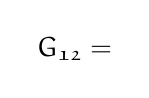
\begin{tikzpicture}[baseline=(current bounding box.center)]
    \node {$G_{\mathfrak{12}}=$};
\end{tikzpicture}
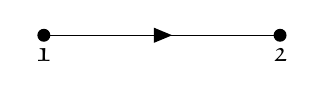
\begin{tikzpicture}[baseline=(current bounding box.base)]
	\begin{feynman}%[inline=(a.base)]
		\vertex[dot] (a) {};
		\vertex[dot, right=3cm of a] (b) {};
		
		\node [below=0.25cm of a] {$\mathfrak{1}$};
		\node [below=0.25cm of b] {$\mathfrak{2}$};
		
		\diagram* {
			(a) -- [fermion] (b)
		};	
	\end{feynman}
\end{tikzpicture}

\end{document}